\chapter*{Organisation du projet}
\addcontentsline{toc}{chapter}{Organisation du projet}
\markboth{Organisation du projet}{Organisation du projet}
\label{sec:organisation}
\section*{Planning}
\addcontentsline{toc}{section}{Planning}
Les figures \ref{fig:mvp-plan}, \ref{fig:gestion-proj} et \ref{fig:r1-plan} montrent le planning que nous allons suivre pour réaliser notre projet.

\begin{figure}[!ht]
	\centering
	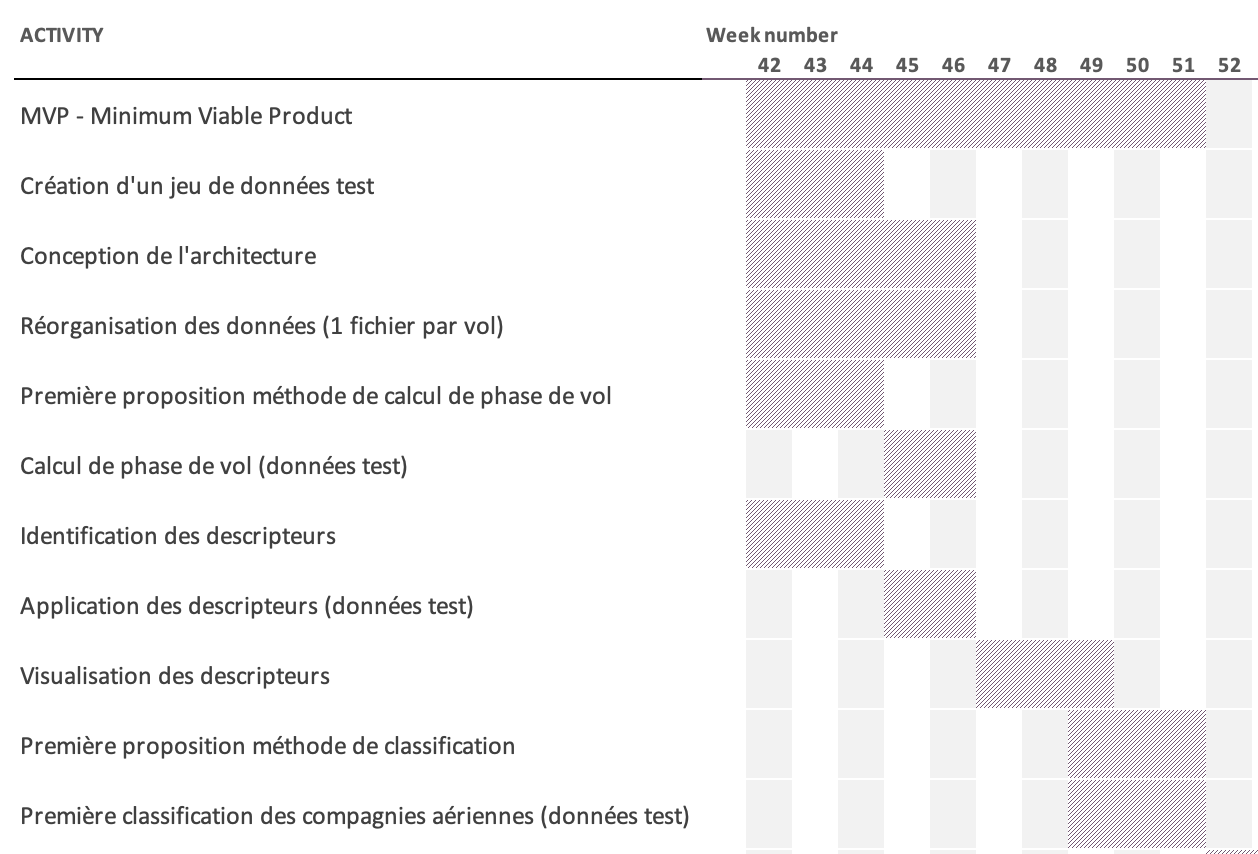
\includegraphics[width=15cm]{MVP planning}
	\caption{planning associé au produit minimal(MVP)}
	\label{fig:mvp-plan}
\end{figure}

\begin{figure}[!ht]
	\centering
	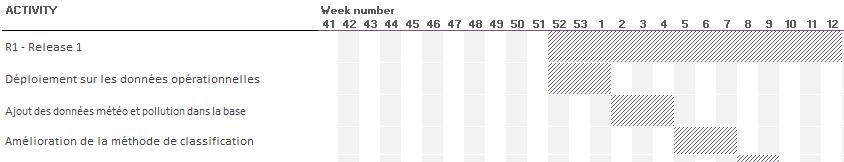
\includegraphics[width=15cm]{R1 planning}
	\caption{planning associé au produit final}
	\label{fig:r1-plan}
\end{figure}

\begin{figure}[!ht]
	\centering
	\includegraphics[width=15cm]{gestion projet}
	\caption{planning associé à la gestion de projet}
	\label{fig:gestion-proj}
\end{figure}

\section*{Association des taches aux membres du projet}
\addcontentsline{toc}{section}{Association des taches aux membres du projet}
La matrice en figure \ref{fig:raci} présente l'attribution des tâches à chaque membre du projet:


\begin{figure}[!h]
	\centering
	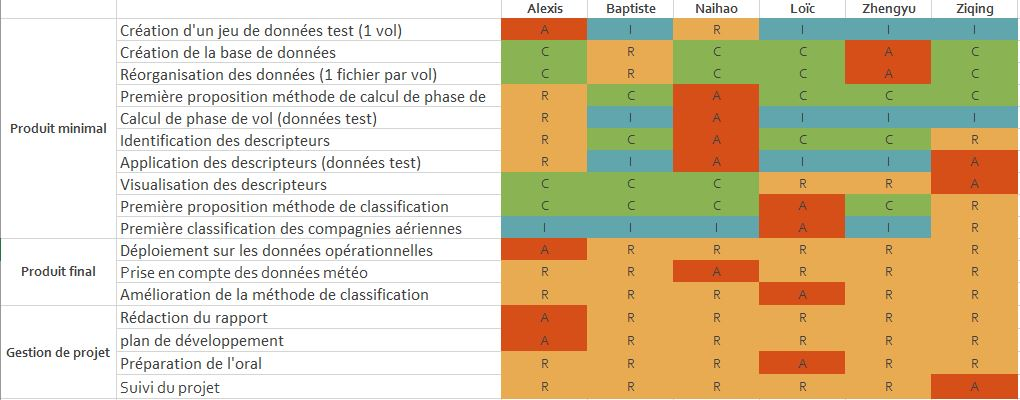
\includegraphics[width=15cm]{RACI}
	\caption{matrice RACI, R:responsible, A:accountable, C:consulted, I:informed}
	\label{fig:raci}
\end{figure}
\section*{Suivi}
\addcontentsline{toc}{section}{Suivi}
Afin que la communication au sein du projet soit de bonne qualité, nous avons mis en place un drive google où sont stockés les documents qui concernent la gestion du projet (cahier charge, compte rendu de réunion,...). Afin d'assurer les travaux de développement et de rédaction de document qui sont souvent fait en équipe, nous avons mis en place un répertoire github. Ces deux répertoires sont accessibles et modifiables depuis n'importe quel poste et par n'importe quel membre du projet. 

Chaque semaine, une réunion sera organisé ce qui permettra de faire un point régulier de l'avancement du projet. Il permettra aussi à chaque membre de poursuivre les tâches qui lui sont attribuées.

D'autre part, nous utiliserons la librairie pandas sous python pour assurer le traitement des données, ainsi que django pour réaliser des applications web. En ce qui concerne la partie gestion de projet, nous utiliserons la suite office ainsi que latex pour rédiger les rendus.

\section*{Organigramme}
\addcontentsline{toc}{section}{Organigramme}
Voici ici l'organigramme correspondant à notre projet.
\begin{figure}[!ht]
	\centering
	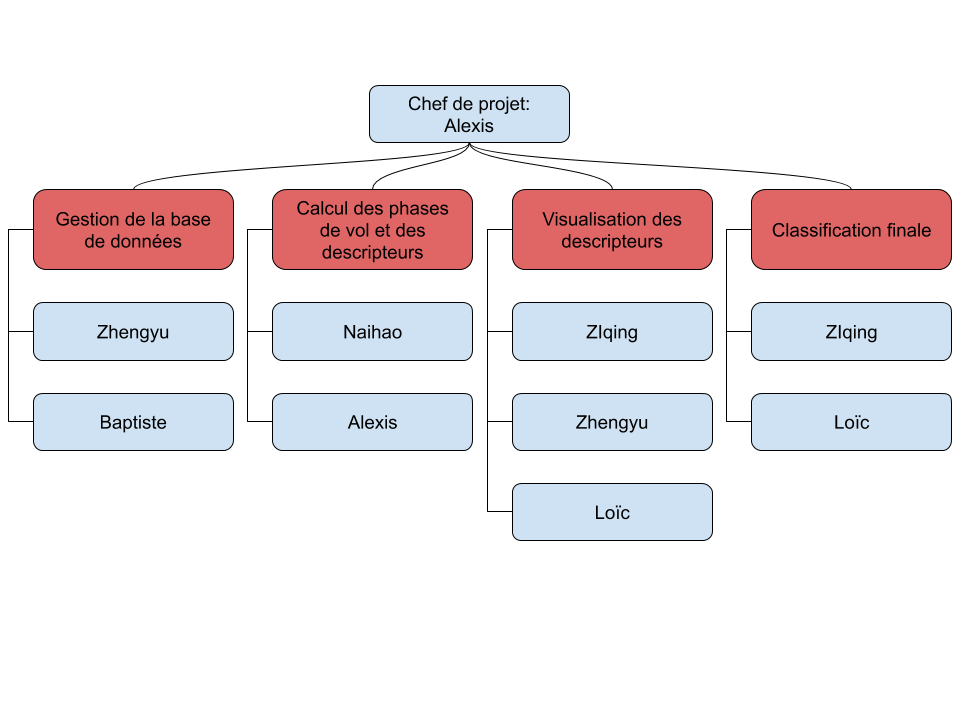
\includegraphics[width=10cm]{Organigramme}
	\caption{Organigramme}
	\label{fig:Organigramme}
\end{figure}


%%% Local Variables: 
%%% mode: latex
%%% TeX-master: "isae-report-template"
%%% End: 